\documentclass[aps,apl,twocolumn,groupedaddress]{revtex4-1}
%\documentclass[12pt]{article}   	% use "amsart" instead of "article" for AMSLaTeX format

\usepackage{graphicx}				% Use pdf, png, jpg, or eps� with pdflatex; use eps in DVI mode
								% TeX will automatically convert eps --> pdf in pdflatex		
%\usepackage{caption}

\begin{document}

\title{A Novel Route to the Semi-Classic Limit of Quantum Mechanics}
\author{Chris Richardson, Peter Schlagheck, John Martin, ?Nicolas Vandewalle?, Thierry Bastin}
\affiliation{University of Liege}
\date{\today}							% Activate to display a given date or no date

\begin{abstract}

%A wave equation which sheds light on the origin of the Schr\"{o}dinger equation has previously been proposed.  This equation which we call the classical Schr\"{o}dinger-like equation is the Schr\"{o}dinger equation plus an extra non-linear term, a classicality-enforcing potential, which has the effect of canceling out all quantum and wave-like effects.  The Schr\"{o}dinger equation has been recovered from the classical Schr\"{o}dinger-like equation by making assumptions which have the effect of completely canceling the classicality-enforcing potential.
%
%We demonstrate both analytically and numerically that it is not strictly necessary to get rid of the classicality-enforcing potential to recover quantum behavior.  We show that by scaling and not necessarily eliminating the classicality-enforcing potential the linear Schr\"{o}dinger equation is recovered, but with a rescaled $\hbar$.  Even though the classical Schr\"{o}dinger-like equation with a scaled classicality-enforcing potential is non-linear, we demonstrate that it behaves in a very linear way.
%
%We call the classical Schr\"{o}dinger-like equation with a scaled classicality-enforcing potential the transition equation and it can be a tool to explore the transition between the quantum and classical worlds.

We present a novel approach to explore the classical limit of quantum theory based on a non-linear classical Schr\"{o}dinger-like equation which includes a classicality enforcing potential.  Scaling of this potential is shown to recover quantum behavior and is equivalent to scaling Plank's constant to the classical limit.

\end{abstract}

\maketitle

\section{Introduction}

The boundary between where quantum mechanics ends and classical mechanics begins is being pushed.  Experiments such as Arndt et al's entangled fullerenes~\cite{bib:arndt} demonstrate quantum behavior on a classical, macroscopic scale.  It is therefore important to be able to describe the manner in which quantum behavior transitions into classical behavior.  Quantum mechanics is an extremely well tested theory and there is no doubt that all the behavior of classical mechanics is contained entirely within quantum theory.  A position that the Ehrentfest theorem backs up by demonstrating that the expected values of measurement predicted from quantum mechanics obey classical Newtonian motion.  However as we push quantum mechanics into the classical domain it becomes increasingly difficult to represent the systems using the full quantum formalism.  It is often unfeasible to a model macroscopic system without somehow approximating quantum mechanics and the Schr\"{o}dinger equation,
\begin{eqnarray}
i \hbar \frac{\partial \psi}{\partial t} &=& - \frac{\hbar^2}{2 m} \nabla^2 \psi + V \psi \;, \label{eqn:schrod}
\end{eqnarray}
where $\psi$ is a wavefunction whose modulus squared gives a probability density, $m$ is the mass, $V$ is the potential and $\hbar$ is Plank's constant.  

Eliminating Plank's constant is an obvious way to get to the classical regime.  It stands to reason that eliminating this purely quantum mechanical term may also eliminate quantum behavior.  But we can immediately see that the Schr\"{o}dinger equation suffers a reduction in order and looses all usefulness.  Another technique, the WKB approximation~\cite{bib:wkb}, approximates solutions to the Schr\"{o}dinger equation with a Plank's constant which is reduced instead of eliminated.  It assumes that the amplitude, $A$, of the wavefunction in its polar form $\psi = A e^{ i S / \hbar }$ where $S$ is the phase, to be slowly varying compared to the phase term $S / \hbar$.  This leads to successful approximate solutions in the semi-classical regime but they become singular near the classical turning point.  In the following we propose a new tool that allows description of the entire transition from the quantum to the classical regimes.

Despite classical mechanics being completely contained in quantum mechanics they are discussed in quite different languages.  To develop a tool that smoothly transitions from the two regimes we must be able to describe them both using the same language.  Quantum mechanics is described by the Schr\"{o}dinger wave equation[cite] a partial differential equation that describes how a quantum state evolves in time.    This wave equation leads to behavior that is never observed in classical mechanics such as single particle interference[cite], entanglement[cite] and wave-particle duality[cite].   Following Madelung~\cite{bib:madelung} and Bohm~\cite{bib:bohm} we can reveal an interesting expression that expresses this unique behavior as a classical potential.  We can use the polar wavefunction form with the Schr\"{o}dinger equation to derive what Bohm coined the \emph{quantum-mechanical potential},
\begin{eqnarray}
U = - \frac{\hbar^2}{2 m} \frac{ \nabla^2 A}{A} = - \frac{\hbar^2}{2 m} \frac{1}{\left| \psi \right|} \nabla^2 \left| \psi \right| \;.\label{eqn:qm_pot}
\end{eqnarray}
This potential added to the the classical Hamilton-Jacobi equation describes a particle that will exhibit all the unique behavior we associate only with quantum mechanics.  This same term appears again when considering how to describe classical mechanics using the same language as quantum mechanics.

The equations of classical mechanics predict deterministic trajectories for given initial conditions.  If we have ensemble of initial conditions we also have a similar ensemble of trajectories which are defined by $A_{cl}$.  A classical wavefuction, $\psi_{cl} = A_{cl} e^{ i S_{cl} / \hbar }$, can be constructed where $S_{cl}$ is the classical action from the Hamilton-Jacobi equation and $\hbar$ is used to provide a dimensionless argument.  Oriols and Mompart~\cite{bib:obm} use this form of the wavefunction to derive a classical wave equation similar to the Schr\"{o}dinger equation that describes evolution of a classical ensemble of trajectories.  We call it the classical Schr\"{o}dinger-like equation and it is defined as
\begin{eqnarray}
i \hbar \frac{\partial \psi_{cl}}{\partial t} &=& - \frac{\hbar^2}{2 m} \nabla^2 \psi_{cl} \nonumber \\
&+& \left(V + \frac{\hbar^2}{2 m} \frac{1}{\left| \psi_{cl} \right|} \nabla^2 \left| \psi_{cl} \right| \right) \psi_{cl} \;,\label{eqn:class_schrod}
\end{eqnarray}
where the probability density, in analogy to quantum mechanics, is given from the modulus squared of $\psi_{cl}$.  Eq.~(\ref{eqn:class_schrod}) while being completely classical is similar to the Schr\"{o}dinger equation except for the extra non-linear term which has the effect of canceling out all quantum or wave-like effects.  Schleich et al. refer to this term as the \emph{classicality-enforcing potential}.  It is of course Bohm's quantum-mechanical potential, Eq.~(\ref{eqn:qm_pot}), with the opposite sign.

Both the classical and quantum regimes can now be described using the same language, that of a wave equations and probabilities, and we can now explore how to transition between the two regimes.  Schleich et al. transfer from the non-linear classical Schr\"{o}dinger-like equation, Eq.~(\ref{eqn:class_schrod}),  to the linear Schr\"{o}dinger equation, Eq.~(\ref{eqn:schrod}), by first making the anzatz $\psi_{cl} = \psi$.   They then associate the classicality-enforcing potential with the quantum action.  In this way, the classicality-enforcing potential is canceled out in Eq.~(\ref{eqn:class_schrod}).  We would like to add, however, that it is not strictly necessary to get rid of the classicality-enforcing potential to recover quantum behavior.  We have found that by scaling and not necessarily eliminating the classicality-enforcing potential we can reproduce quantum behavior and recover the linear Schr\"{o}dinger equation with a rescaled $\hbar$.  We do this by inserting a degree of quantumness, $0 \leq \epsilon \leq 1$, into Eq.~(\ref{eqn:class_schrod}) which allows us to explore the smooth transition from the classical world, $\epsilon = 0$, to the quantum one, $\epsilon = 1$.

\begin{eqnarray}
i \hbar \frac{\partial \psi}{\partial t} &=& - \frac{\hbar^2}{2 m} \nabla^2 \psi \nonumber \\ 
&+& \left(V + (1 - \epsilon) \frac{\hbar^2}{2 m} \frac{1}{\left| \psi \right|} \nabla^2 \left| \psi \right| \right) \psi\label{eqn:class_schrod_ep}
\end{eqnarray}

We call this the transition equation and we will show that for all values of $\epsilon \neq 0$ it exhibits quantum behavior.  To demonstrate this we take two approaches.  First in Sec.~\ref{sec:scaling} we show analytically that the transition equation is equivalent to the Schr\"{o}dinger equation with a rescaled $\hbar$.  We then in Sec.~\ref{sec:inter} explore numerically what the effect of scaling the classicality-enforcing potential has on the interference of two Gaussian wave packets.

\section{Equivalence to Scaling Plank's Constant\label{sec:scaling}}

The non-linear transition equation can be shown to be equivalent to the linear Schr\"{o}dinger equation with a $\hbar$ scaled by the degree of quantumness,
\begin{eqnarray}
\tilde{\hbar} = \hbar \sqrt{\epsilon} \;. \label{eqn:hbar_scaled}
\end{eqnarray}

We begin by inserting the polar form of the wave equation into the transition equation, Eq.~(\ref{eqn:class_schrod_ep}), and finding the individual elements.  The Laplacian is found to be
\begin{eqnarray}
\nabla^2 \psi &=& \big[ \nabla^2 A + 2 \frac{i}{\hbar}  (\nabla A) \cdot (\nabla S) \nonumber \\
&+& \frac{i}{\hbar} A \nabla^2 S - \frac{1}{\hbar^2}  A (\nabla S)^2 \big] e^{ i S / \hbar } \;.
\end{eqnarray}

The time derivative of the polar wavefunction is
\begin{eqnarray}
i \hbar \frac{\partial \psi}{\partial t} &=& (i \hbar \frac{\partial A}{\partial t} - A \frac{\partial S}{\partial t}) e^{ i S / \hbar } \;.
\end{eqnarray}

The contribution from the classicality-enforcing potential is
\begin{eqnarray}
\frac{\psi}{\left| \psi \right|} \nabla^2 \psi &=& (\nabla^2 A) e^{ i S / \hbar } \;.
\end{eqnarray}

Gathering the real and imaginary terms we recover two equations.  The first is the standard continuity equation which enforces the conservation of probability
\begin{eqnarray}
\frac{\partial A}{\partial t} &=& - \frac{1}{m} (\nabla A) \cdot (\nabla S) - \frac{1}{2 m} A \nabla^2 S \;, \label{eqn:continuity} \\
&=& i \frac{\hbar}{2 m} \frac{1}{2 A} \nabla \cdot (\psi^* \nabla \psi - \psi \nabla \psi^*) =  - \frac{1}{2 A} \nabla \cdot \vec{j} \;, \\
0 &=& \frac{\partial \rho}{\partial t} + \nabla \cdot \vec{j} \;,
\end{eqnarray}
where $\frac{\partial \rho}{\partial t}  =\frac{\partial  \left| \psi \right|^2}{\partial t} =  2 A \frac{\partial  A}{\partial t}$ and $\vec{j}$ is the probability current.  The second is an equation very similar to the Hamilton-Jacobi equation.  It differs by the addition of the quantum-mechanical potential, Eq.~(\ref{eqn:qm_pot}) , scaled by the degree of quantumness,
\begin{eqnarray}
 \frac{\partial S}{\partial t} &=& - \frac{1}{2 m} (\nabla S)^2 - V + \epsilon \frac{\hbar^2}{2 m} \frac{ \nabla^2 A}{A} \;.
\end{eqnarray}

This equation can be made to have the appearance of the Schr\"{o}dinger equation by making the substitution $\tilde{\hbar} = \hbar \sqrt{\epsilon}$.   Performing this substitution yields
\begin{eqnarray}
\frac{\partial S}{\partial t} &=& - \frac{1}{2 m} (\nabla S)^2 - V + \frac{\tilde{\hbar}^2}{2 m} \frac{ \nabla^2 A}{A} \;,\label{eqn:hamilton-jacobi_rescaled}
\end{eqnarray}
which has had the effect of canceling out the degree of quantumness.  Eqs.~(\ref{eqn:continuity}) and (\ref{eqn:hamilton-jacobi_rescaled}) are now completely equivalent to the Schr\"{o}dinger equation with a rescaled $\hbar$ and we can write
\begin{eqnarray}
\psi &=& A e^{i S / \tilde{\hbar}} \;, \\
i \tilde{\hbar} \frac{\partial \psi}{\partial t}  &=& -  \frac{\tilde{\hbar}^2}{2 m} \nabla^2 \psi + V \psi \;.
\end{eqnarray}
 
\section{The Interference of Two Wave Packets\label{sec:inter}}

Using quantum mechanics we would expect two wave packets to spread with time and then to be represented by the standard Young interference pattern~\cite{bib:Young}.  For classical particles with no wave nature we expect the particles to behave like baseballs and pass through one or the other slit and continue on without diffraction for all time.  We can explore the transition between these two extremes by solving the non-linear transition equation numerically.  For comparison, we first solve the system using the fully quantum Schr\"{o}dinger equation.

\subsection{Fully Quantum Wave Packets}

\begin{figure*}[ht]
\begin{minipage}[t]{0.32\textwidth}
%\centering
  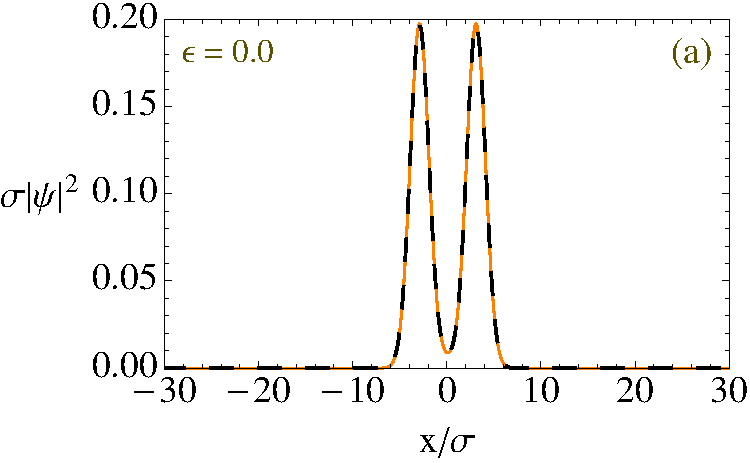
\includegraphics[width=1\textwidth]{Graphics/Probs_ep-10.pdf}
  %\caption*{(a)}
\end{minipage}
\begin{minipage}[t]{0.32\textwidth}
%\centering
  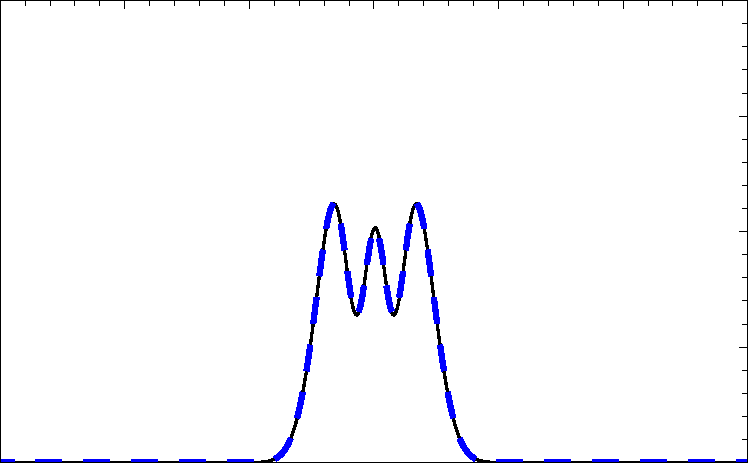
\includegraphics[width=1\textwidth]{Graphics/Probs_ep-98.pdf}
  %\caption*{(b)}
\end{minipage}
\begin{minipage}[t]{0.32\textwidth}
%\centering
  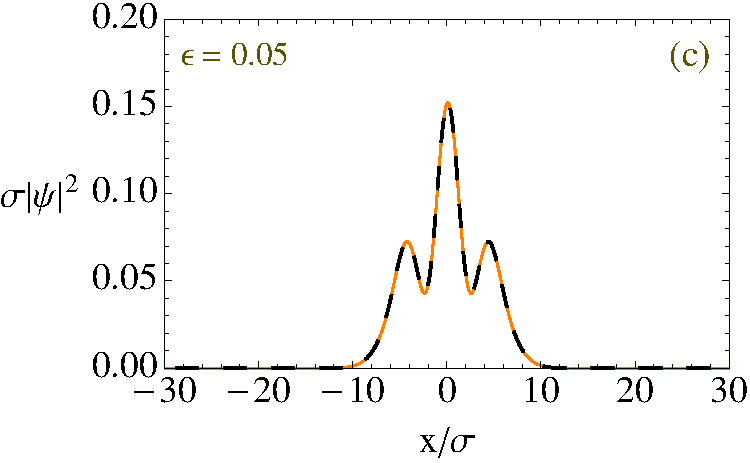
\includegraphics[width=1\textwidth]{Graphics/Probs_ep-95.pdf}
  %\caption*{(c)}
\end{minipage}
\begin{minipage}[t]{0.32\textwidth}
%\centering
  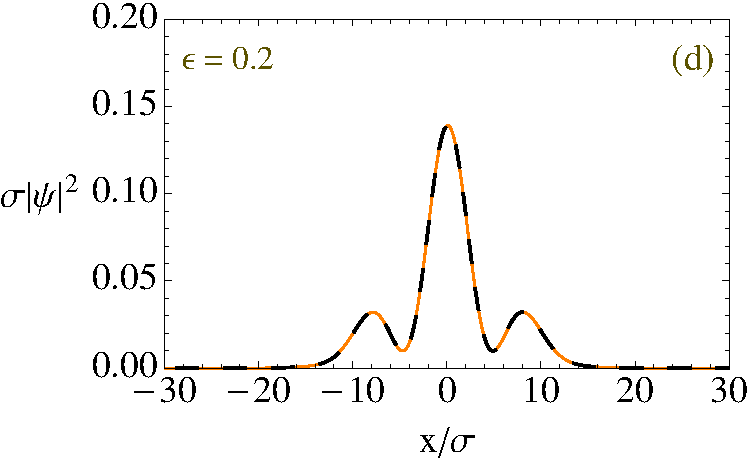
\includegraphics[width=1\textwidth]{Graphics/Probs_ep-8.pdf}
  %\caption*{(d)}
\end{minipage}
\begin{minipage}[t]{0.32\textwidth}
%\centering
  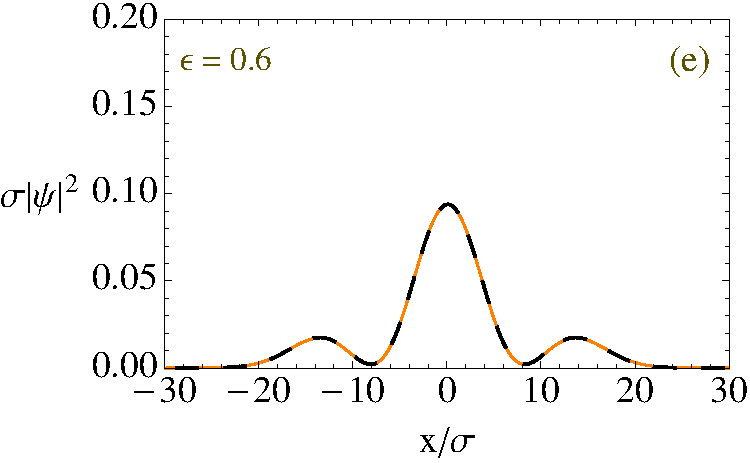
\includegraphics[width=1\textwidth]{Graphics/Probs_ep-4.pdf}
  %\caption*{(e)}
\end{minipage}
\begin{minipage}[t]{0.32\textwidth}
%\centering
  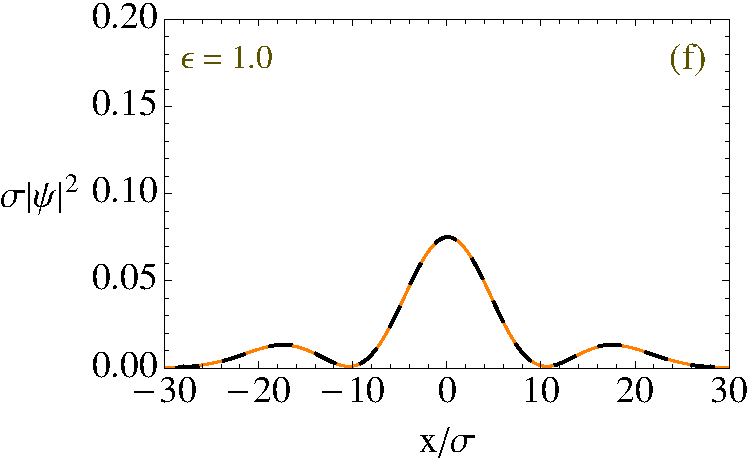
\includegraphics[width=1\textwidth]{Graphics/Probs_ep-0.pdf}
  %\caption*{(f)}
\end{minipage}
\caption{Solid line is the analytic probability density using the Schr\"{o}dinger equation with a scaled $\hbar = \tilde{\hbar} \sqrt{\epsilon}$ and the dashed line is the simulated probability density using the transition equation.  All plots are evaluated at the same time $t = 20 \frac{m \sigma^2}{\hbar}$ and the distance between the center of the two gaussians is $d = 6 \sigma$. Plot (a) is the fully classical case with $\epsilon = 0$. (b) $\epsilon = 0.02$. (c) $\epsilon = 0.05$. (d) $\epsilon = 0.2$. (e) $\epsilon = 0.6$. (f) is for the case $\epsilon = 1$ when $\tilde{\hbar} = \hbar$.}
\label{fig:diffract_movie}
\end{figure*}

We start the quantum analysis with two gaussians in one dimension with $V = 0$ and initial conditions
\begin{eqnarray}
i \hbar \frac{\partial \psi}{\partial t} &=& -\frac{\hbar^2}{2 m} \frac{\partial^2 \psi}{\partial x^2} \;.  \\
\psi(x,0) &=& \sqrt{N_0} \left( e^{-\frac{(x-d)^2}{4 \sigma^2}}+e^{-\frac{(x+d)^2}{4 \sigma ^2}}\right) \label{eqn:double_init}
\end{eqnarray}
where $d$ is the distance from the origin to the centers of the Gaussians and $\sigma$ is the root mean square (rms) width. The normalization is
\begin{eqnarray}
 N_0 = 1 / \left(2 \sqrt{2 \pi } \sigma  \left(e^{-\frac{d^2}{2 \sigma ^2}}+1\right)\right) \;.
 \end{eqnarray}

When the time-dependent Schr\"{o}dinger is solved for the initial condition, Eq.~(\ref{eqn:double_init}), the time-dependent wave function is found to be
\begin{eqnarray}
\psi(x,t) &=& \sqrt{\frac{N_0}{a_t}} \left(e^{-\frac{(x-d)^2}{4 a^2_t}}+e^{-\frac{(x+d)^2}{4 a^2_t}}\right) \;.
\end{eqnarray}
where $a^2_t = 1+i \frac{\hbar}{2 m \sigma^2} t$.  When the modulus is squared the interference term becomes obvious.

\begin{eqnarray}
\left| \psi(x,t) \right|^2 &=& \frac{N_0}{\sigma_t} \Bigg[\left(e^{-\frac{(x-d)^2}{4 \sigma^2_t}}+e^{-\frac{(x+d)^2}{4 \sigma^2_t}}\right)^2 \label{eqn:wf_double_t} \nonumber \\
&-& 4 e^{-\frac{ \left(x^2 + d^2\right)}{2 \sigma^2_t}} \sin^2 \left(\frac{\hbar}{4 m \sigma^2 \sigma^2_t} t x d \right)\Bigg]\end{eqnarray}
where $\sigma^2_t = \frac{\hbar^2}{4 m^2 \sigma^2} t^2 +\sigma^2$ is the time dependent rms width.  This gives the expected Young interference pattern as can be seen in Fig.~(\ref{fig:diffract_movie}-f).

\subsection{The Semi-Quantum Semi-Classical Wave Packets}

To explore the transitional behavior of the interference of two Gaussian wave packets from the quantum to the classical regime we use the transition equation, Eq.~(\ref{eqn:class_schrod_ep}), in one dimension and with $V = 0$
\begin{eqnarray}
i \hbar \frac{\partial \psi}{\partial t} &=& -\frac{\hbar^2}{2 m} \frac{\partial^2 \psi}{\partial x^2} + (1 - \epsilon) \frac{\hbar^2}{2 m} \frac{\psi}{\left| \psi \right|} \frac{\partial^2 \left| \psi \right|}{\partial x^2} \;.  \label{eqn:schrod_class_nov}
\end{eqnarray}

This equation can be solved numerically using the explicit finite difference method.  To do so Eq.~(\ref{eqn:double_init}) is discretized into $\psi_{x_n,0}$ where $x_n = n \Delta x$.  The next time step, $t_n = n \Delta t$, for Eq.~(\ref{eqn:schrod_class_nov}) is given by the recurrence relation
\begin{eqnarray}
\psi(x_n,t_{n+1}) &=& i \frac{\Delta t}{(\Delta x)^2} \Big[ \psi_{x_{n+1},t_n} + \psi_{x_{n-1},t_n} \nonumber \\
&-& \psi_{x_n,t_n} \left(2 + i \frac{(\Delta x)^2}{\Delta t}\right) \nonumber \\
&-& (1 - \epsilon) \frac{\psi_{x_n,t_n}}{\left|\psi_{x_n,t_n}\right|} \Big(\left| \psi_{x_{n+1},t_n} \right| \nonumber \\
&-&  2 \left| \psi_{x_n,t_n} \right| + \left| \psi_{x_{n-1},t_n} \right| \Big)\Big] \;.
\end{eqnarray}
The asymptotic behavior is as expected.  For the completely quantum case, $\epsilon = 1$, the interference pattern that forms, Fig.~(\ref{fig:diffract_movie}-f), is identical to the analytic case, Eq.~(\ref{eqn:wf_double_t}).  For the completely classical case, $\epsilon = 0$, the interference pattern that forms, Fig.~(\ref{fig:diffract_movie}-a), is just that of the initial distribution, Eq.~(\ref{eqn:double_init}).  As can be seen in all the frames of Fig.~(\ref{fig:diffract_movie}) for all values of $\epsilon$ the numerically solved non-linear transition equation is equivalent to the linear Schr\"{o}dinger equation with a scaled $\hbar$
%
%For all values of $0 < \epsilon \leq 1$, given enough time, a far-field diffraction pattern will develop with a visibility of one.  The time for a diffraction pattern to develop increases to infinity as degree of quantumness diminishes, $\epsilon \rightarrow 0$.  The diffraction patterns for the higher values of $\epsilon$ are less developed that for the lower values, but the visibility for all of them is one.

For all values of $0 < \epsilon \leq 1$ an interference pattern develops.  Given enough time the pattern will develop into the usual far-field Young interference pattern with a visibility of one.  As can be seen in Fig.~(\ref{fig:diffract_movie}) the time for a diffraction pattern to develop increases to infinity as degree of quantumness diminishes.  The only value in which no interference is observed is that for $\epsilon = 0$.  When using the transition equation classical mechanics is a special singular case.

\section{Conclusion}
\subsection{Restate Everything and Comment on Linearity}
We have demonstrate both analytically and numerically that it is not necessary to get rid of the classicality-enforcing potential to recover quantum behavior.  We have found that by scaling and not necessarily eliminating the classicality-enforcing potential quantum behavior is observed and the linear Schr\"{o}dinger equation is recovered, but with a rescaled $\hbar$.  We can scale the degree of quantumness in the transition equation to explore the transition are between the classical and quantum worlds.  This does leave us with a non-linear equation to solve, but it avoids the problems that arise when approximating the Schr\"{o}dinger equation with a reduced Plank's constant.  It is interesting that the unique behavior of a linear theory like quantum mechanics can be reproduced with a non-linear wave equation.  It has been well proven in many experiments [cite] that quantum mechanics is linear and so too is the transition equation with a vanishing degree of quantumness.  However when the degree of quantumness rises above zero quantum behavior is observed.  The non-linear transition equation mimics the linear Schr\"{o}dinger equation.
  
\subsection{Classical Mechanics is Singular and a Relaxation of Requirements}
It is interesting that pure classical mechanics is only observed for the singular case when the degree of quantumness vanishes completely.  It is more natural to have quantum effects than not.  This is evident when observing the microscopic world as it is very difficult to avoid quantum effects.  It is less obvious for macroscopic experiments, where quantum behavior should be absent.  When these experiments are considering in the light of the transition equation it should be noted that quantum behavior is almost never absent and it only needs be teased out.  For experiments that operate in the transition area it is therefore not necessary to make a one-to-one correspondence with quantum mechanics to demonstrate quantum behavior.  The transition equation allows a relaxation of the requirements that an experiment would have abide by to be able to definitively say that quantum behavior was observed.

\subsection{Same Language and Quandrops}
The classical Schr\"{o}dinger-like equation allows us to describe quantum and classical mechanics using the same language.  Surprisingly there is a system, Quandrops, which is purely classical and macroscopic but which nevertheless displays quantum-like behavior.

\begin{acknowledgments}
We would like to thank the Action de Recherche Concert�e (ARC) and the rest of the Quandrops team.
\end{acknowledgments}

\begin{thebibliography}{4}

\bibitem{bib:arndt}
M. Arndt, O. Nairz, J. Vos-Andreae, C. Keller, G. van der Zouw, and A. Zeilinger, \emph{Waveparticle duality of C60 molecules}, Nature 401, 680 (1999).

\bibitem{bib:newton}
Newton, Isaac, \emph{Philosophiae Naturalis Principia Mathematica}, London, (1687).

\bibitem{bib:hamiltonjacobi}
Landau, L. D. and Lifshitz, E. M., \emph{Mechanics}, Pergamon Press, Oxford, (1969).

\bibitem{bib:macent}
S. Ghosh, T. F. Rosenbaum, G. Aeppli and S. N. Coppersmith, \emph{Entangled quantum state of magnetic dipoles}, Nature 425 48 (2003).

\bibitem{bib:bohm}
D. Bohm, \emph{A Suggested Interpretation of the Quantum Theory in Terms of ``Hidden'' Variables}. I, Phys. Rev. 85, 166 (1952).

\bibitem{bib:madelung}
E. Madelung, \emph{Quantentheorie in hydrodynamischer}. Z Phys 40:322�326. (1926).

\bibitem{bib:wkb}
Sakurai, J. J., \emph{Modern Quantum Mechanics. Addison-Wesley}, (1993)

\bibitem{bib:obm}
X.Oriols and J.Mompart \emph{Overview of Bohmian Mechanics}pages: 15-147; Chapter 1 of the book \emph{Applied Bohmian Mechanics: From Nanoscale Systems to Cosmology} Editorial Pan Stanford Publishing Pte. Ltd (2012).

\bibitem{bib:revisited}
Wolfgang P. Schleich, Daniel M. Greenberger, Donald H. Kobe, and Marlan O. Scully
\emph{Schr\"{o}dinger equation revisited}
PNAS 2013 110 (14) 5374-5379; published ahead of print March 18, 2013, doi:10.1073/pnas.1302475110

\bibitem{bib:Young}
Thomas Young, emph{Experimental Demonstration of the General Law of the Interference of Light, Philosophical Transactions of the Royal Society of London}, vol 94 (1804).

\bibitem{bib:couder_orbits}
E. Fort, A. Eddi, A. Boudaoud, J. Moukhtar, and Y. Couder, \emph{Path-memory induced quantization of classical orbits}, PNAS 107, 17515 (2010).

\bibitem{bib:theonlymystery}
Feynman, Richard P. \emph{Six Easy Pieces} Reading, MA: Addison-Wesley, 1995.

\end{thebibliography}


\end{document}  